\section{Results} \label{results}

Data collection took place between February and June 2023 through the British online platform Prolific, with all participants recruited from the United Kingdom.\footnote{EXCLUSION CRITERIA: leave a comment for Felix to insert later} A total of $322$ subjects were recruited ($161$ assigned to Player~A, $161$ to Player~B).\footnote{We preregistered the collection of data from $320$ participants ($80$ subjects per role per treatment). Due to attrition and subsequent re-matching we recruited an extra pair in the \textit{Punishment} condition.} On average, Player~A spent $12$ minutes completing the experiment and earned an average bonus of $\pounds 2.49$ on top of the Prolific show-up fee, while Player~B spent approximately $8$ minutes and earned an average bonus of $\pounds 2.30$. Treatment randomization was effective, as demonstrated by the balance across observable characteristics (Appendix~\ref{appendix:sum_stats}, Table~\ref{tab:treatment_balance}). A flow diagram showing recruitment, attrition, attention-check exclusion, and the analysis sample, broken down by condition and role, appears in Appendix~\ref{appendix:attrition}; in particular, attrition rates do not differ meaningfully across the \textit{Punishment} and \textit{No-Punishment} conditions.

We preregistered exclusion of subjects who failed the attention check on the screen at which their main outcome variable was elicited. For Player~A, this is the belief-elicitation screen; for Player~B, the punishment-elicitation screen. Of $161$ Player~Bs, $135$ pass the attention check ($83.9\%$); the corresponding pass rate for Player~A is $131/161$ ($81.4\%$). All main results are robust to including subjects who fail the attention check; we report these robustness checks in Appendix~\ref{appendix:regs}.
\todo[inline]{FB: maybe move to first set of results. Also the appendix does not show anything and the default should be including everyone.}

\subsection*{Result~1: Punishment reduces delegation} \label{sec:result1}

\paragraph{Headline.} In the \textit{Punishment} condition, where Player~B can punish, $42.5\%$ of Player~As delegated the decision to the algorithm. In the \textit{No-Punishment} condition, where punishment is impossible, $59.3\%$ delegated. Figure~\ref{fig:delegation_shares} illustrates the difference. The introduction of potential punishment thus significantly \textit{reduces} the likelihood of delegation to the algorithm (Pearson Chi-squared, $p=0.033$; Fisher's exact, $p=0.041$).\footnote{The preregistration is non-directional on H1; the realized direction is opposite to that anticipated by the responsibility-avoidance literature on which the hypothesis was grounded. We report two-sided tests throughout the body of the paper. The full set of preregistered tests, the deviations from each, and the rationale appears in Appendix~\ref{appendix:preregistration}.}\footnote{A within-subject corroborator points the same direction. Player~As in the \textit{No-Punishment} condition were asked, after their actual delegation decision, the hypothetical question of whether they would have delegated had punishment been possible. Among the $81$ respondents, $12$ would have stopped delegating under hypothetical punishment while only $5$ would have started, yielding a hypothetical delegation rate of $50.6\%$ (within-subject McNemar's test $p=0.090$). Hypothetical responses elicited after the actual decision are subject to motivated reasoning; the within-subject pattern complements rather than substitutes for the between-subject test.}

\medskip
\noindent\textbf{Result~1.} \textit{The possibility of punishment significantly reduces the likelihood that Player~A delegates the decision to the algorithm.}
\medskip

\begin{figure}[!htbp]
    \centering
    \caption{Delegation shares by condition}
    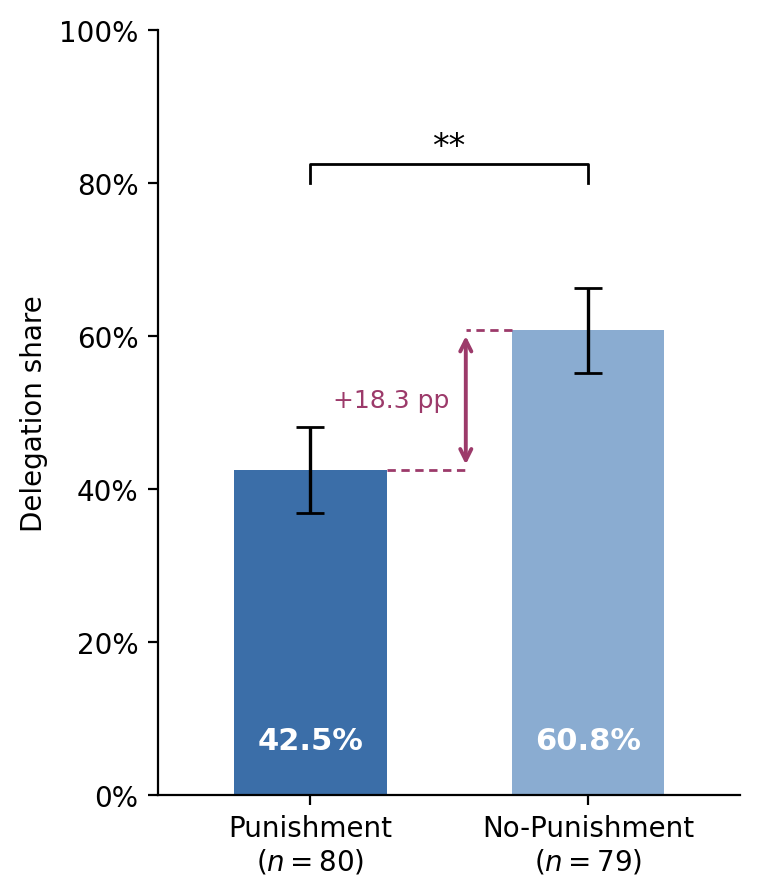
\includegraphics[width=0.5\linewidth]{figures/delegation_shares.png}
    \label{fig:delegation_shares}
    \begin{minipage}{0.6\linewidth}
    \footnotesize
    \textit{Note:} Bars show the share of Player~As who delegated the final prediction to the algorithm in each between-subject condition. The two-sided difference is significant at the $5\%$ level under both a Pearson Chi-squared test ($p=0.033$) and a Fisher's exact test ($p=0.041$). The preregistration does not specify a test direction; the realized effect reverses the sign anticipated by the responsibility-avoidance literature on which the hypothesis was grounded.
    \end{minipage}
\end{figure}

This result not only fails to support \textit{Hypothesis~1}; it points in the opposite direction. The responsibility-avoidance literature, on which H1 rests, would predict the introduction of punishment to make delegation \textit{more} attractive as a tool for shifting responsibility. We instead observe a sizeable reduction in delegation when punishment is on the table. Before turning to candidate mechanisms for this reversal in Section~\ref{sec:mechanism}, we first establish that the effect is robust and document its empirical structure.

\paragraph{With controls.} Table~\ref{tab:del_decision_determinants} reports estimates from a Logit model of the delegation decision. Column~(1) reports the unconditional treatment effect; Column~(2) adds Player~A's task performance and a vector of socio-demographic and technology-affinity controls. The treatment effect is robust: the coefficient on the \textit{No-Punishment} indicator is $0.68$ ($p=0.034$, two-sided) in the unconditional specification and $0.76$ ($p=0.023$, two-sided) with controls. The full set of estimated coefficients is reported in Appendix Table~\ref{tab:reg_delegation}.

\begin{table}[!htbp]
\centering
\scriptsize
\caption{Determinants of the delegation decision}
\label{tab:del_decision_determinants}
\begin{tabular}{@{\extracolsep{5pt}}lcccc|c}
\\[-1.8ex]\hline
\hline \\[-1.8ex]
& \multicolumn{5}{c}{Dependent variable: \textit{Delegation}}\\[0.1cm]
& \multicolumn{4}{c}{\textit{Full sample}} & \textit{Passers} \\
\\[-1.8ex] & (1) & (2) & (3) & (4) & (5) \\
\hline \\[-1.8ex]
 Punishment indicator & $-0.423^{**}$ & $-0.435^{**}$ & $-0.472^{**}$ & $-0.448^{**}$ & $-0.517^{**}$ \\
  & $(0.199)$ & $(0.204)$ & $(0.206)$ & $(0.205)$ & $(0.230)$ \\[0.1cm]
 Task performance &  &  & $-0.119$ &  & $-0.158^{*}$ \\
  &  &  & $(0.079)$ &  & $(0.086)$ \\[0.1cm]
 Perceived performance &  &  &  & $-0.072$ &  \\
  &  &  &  & $(0.056)$ &  \\[0.1cm]
 Age &  & $-0.002$ & $-0.002$ & $-0.002$ & $0.002$ \\
  &  & $(0.009)$ & $(0.009)$ & $(0.009)$ & $(0.010)$ \\[0.1cm]
 Female &  & $0.175$ & $0.222$ & $0.212$ & $0.407$ \\
  &  & $(0.227)$ & $(0.228)$ & $(0.229)$ & $(0.254)$ \\[0.1cm]
 Socio-economic status &  & $-0.038$ & $-0.035$ & $-0.031$ & $-0.082$ \\
  &  & $(0.071)$ & $(0.072)$ & $(0.071)$ & $(0.079)$ \\[0.1cm]
 Went to uni &  & $0.036$ & $0.059$ & $0.025$ & $0.124$ \\
  &  & $(0.227)$ & $(0.225)$ & $(0.227)$ & $(0.247)$ \\[0.1cm]
 Technology score &  & $-0.069$ & $-0.048$ & $-0.062$ & $0.014$ \\
  &  & $(0.092)$ & $(0.095)$ & $(0.092)$ & $(0.107)$ \\[0.1cm]
 Leadership position &  & $0.404^{*}$ & $0.422^{*}$ & $0.399^{*}$ & $0.253$ \\
  &  & $(0.225)$ & $(0.226)$ & $(0.225)$ & $(0.253)$ \\[0.1cm]
 Constant & $0.234^{*}$ & $0.452$ & $0.714$ & $0.716$ & $0.651$ \\
  & $(0.141)$ & $(0.545)$ & $(0.584)$ & $(0.593)$ & $(0.656)$ \\[0.1cm]
\hline \\[-1.8ex]
 AME of Punishment (pp) & $-16.8^{**}$ & $-16.8^{**}$ & $-18.0^{**}$ & $-17.2^{**}$ & $-19.4^{**}$ \\
  & $(p=0.031)$ & $(p=0.030)$ & $(p=0.019)$ & $(p=0.026)$ & $(p=0.021)$ \\
 N & $161$ & $159$ & $159$ & $159$ & $130$ \\
 Pseudo $R^2$ & $0.020$ & $0.039$ & $0.049$ & $0.047$ & $0.064$ \\
\hline
\hline \\[-1.8ex]
\multicolumn{6}{c}{\begin{minipage}{0.85\textwidth}\footnotesize \textit{Note:} Coefficients from a Probit regression of the delegation decision on the Punishment indicator and a set of controls. Robust (HC1) standard errors in parentheses. Significance: $^{*}\,p<0.10$; $^{**}\,p<0.05$; $^{***}\,p<0.01$ (two-sided). Due to missing socio-demographic data, two subjects are dropped in Columns~(2)--(5). The \textit{AME of Punishment} reports the average change in the predicted probability of delegation from introducing the punishment possibility, in percentage points.\end{minipage}}
\end{tabular}
\end{table}


\paragraph{Robustness.} The treatment effect survives several further checks. First, controlling for Player~A's overconfidence (defined as the weighted-average belief about own performance minus actual performance) leaves the \textit{No-Punishment} coefficient essentially unchanged ($0.77$, $p=0.022$); overconfidence itself is not significantly associated with delegation ($p=0.272$). Second, order effects are localised to the \textit{Punishment} condition: presenting the algorithm option first roughly doubles delegation ($52.5\%$ vs $32.5\%$ when the own-decision option is first; $\chi^2$ $p=0.070$), while the \textit{No-Punishment} condition shows no order effect ($p=0.674$); the treatment $\times$ order interaction is not significant ($p=0.115$), so the H1 finding is not driven by interaction with order. Third, relaxing the preregistered attention-check exclusion does not change the result. The full robustness specification is reported in Appendix Table~\ref{tab:reg_delegation_robustness}.

\paragraph{Heterogeneity by performance.} Within the \textit{Punishment} condition, Player~As who performed better on the first ten rounds were less likely to delegate. The Pearson correlation between the score in the first ten rounds and the probability of delegation is $-0.19$ (two-sided $p=0.092$); the corresponding regression coefficient in Column~(3) of Table~\ref{tab:del_decision_determinants} is $-0.61$ (two-sided $p=0.010$). The strengthening of the relationship in the regression reflects, in part, the attention-check restriction (Column~(3) is identified off $n=60$ Punishment-attention-pass subjects, while the raw correlation uses all $80$ Punishment subjects). In the \textit{No-Punishment} condition, no comparable relationship between performance and delegation is observed. Figure~\ref{fig:performance_delegation_scatter} visualises this asymmetry. We flag this paragraph as the empirical hint that motivates the process-ownership mechanism developed in Section~\ref{sec:mechanism}: the condition effect is concentrated among Player~As who, conditional on punishment being on the table, prefer to take a personal stake in producing a good outcome for Player~B.

\begin{figure}[!htbp]
    \centering
    \caption{Delegation share by performance and condition}
    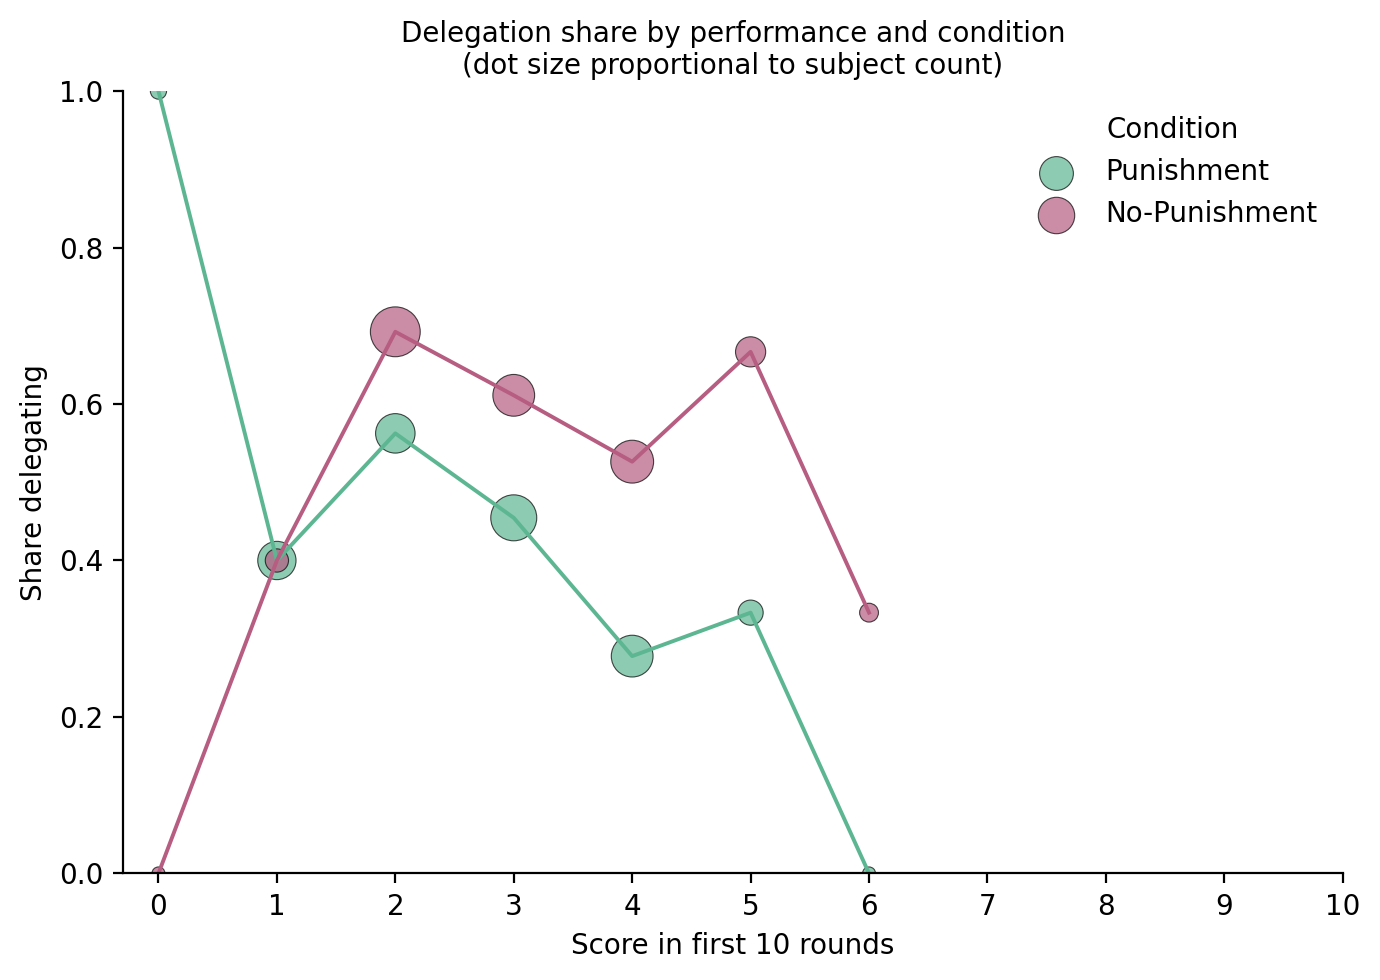
\includegraphics[width=0.7\linewidth]{figures/performance_delegation_scatter.png}
    \label{fig:performance_delegation_scatter}
    \begin{minipage}{0.85\linewidth}
    \footnotesize
    \textit{Note:} Each point reports the share of Player~As at the corresponding first-ten-rounds score who delegated the final prediction. Dot size is proportional to the number of subjects at that score. The downward slope in the \textit{Punishment} condition is the Pearson $r=-0.19$ ($p=0.092$); no comparable slope in \textit{No-Punishment}. Restricted to attention-check passers.
    \end{minipage}
\end{figure}

\subsection*{Result~2: We cannot reject equal punishment of delegated and self-made decisions} \label{sec:result2}

\paragraph{Headline.} We now turn to Player~B's punishment behavior in the \textit{Punishment} condition. Punishment in all four (delegation, outcome) cells of the strategy method is significantly greater than zero, and Player~Bs punish more for low-payoff outcomes than for high-payoff outcomes---an indication that punishment carries informational content rather than being noise; $41.8\%$ of Player~Bs nonetheless do not punish in any of the four scenarios. Conditional on the outcome, however, Player~A is not significantly differently punished depending on the delegation decision. When Player~B receives the high payoff, average punishment is $\pounds 0.311$ for delegated decisions and $\pounds 0.310$ for self-made decisions---a difference of one-tenth of a penny. When Player~B receives the low payoff, average punishment is $\pounds 0.494$ when Player~A delegated versus $\pounds 0.571$ when she made the decision herself; this difference points in the H2 direction but is far from significant (paired $t$-test $p=0.153$; Wilcoxon signed-rank $p=0.533$). The same picture obtains when measuring punishment frequencies rather than amounts: Player~Bs neither punish delegated decisions more harshly, nor do they punish them more frequently (Appendix Figure~\ref{fig:punishment_frequencies}). As preregistered, the within-subject test is identified off the $67$ Player~Bs in the \textit{Punishment} condition who passed the attention check; the result is essentially identical when these subjects are included (mean difference $\pounds 0.071$ vs $\pounds 0.077$; paired $t$-test $p=0.131$ vs $p=0.153$; Appendix Table~\ref{tab:reg_punishment_robustness}).

\medskip
\noindent\textbf{Result~2.} \textit{Conditional on the outcome for Player~B, we cannot reject the hypothesis that Player~A is punished equally for delegated and self-made decisions. A TOST equivalence test rules out moderate insulation effects (those exceeding $\pounds 0.20$, or $10\%$ of the maximum punishment) at $\alpha = 0.05$, but we cannot rule out smaller insulation effects.}
\medskip

\begin{figure}[!htbp]
    \centering
    \caption{Punishment by Player~B and beliefs about punishment by Player~A}
    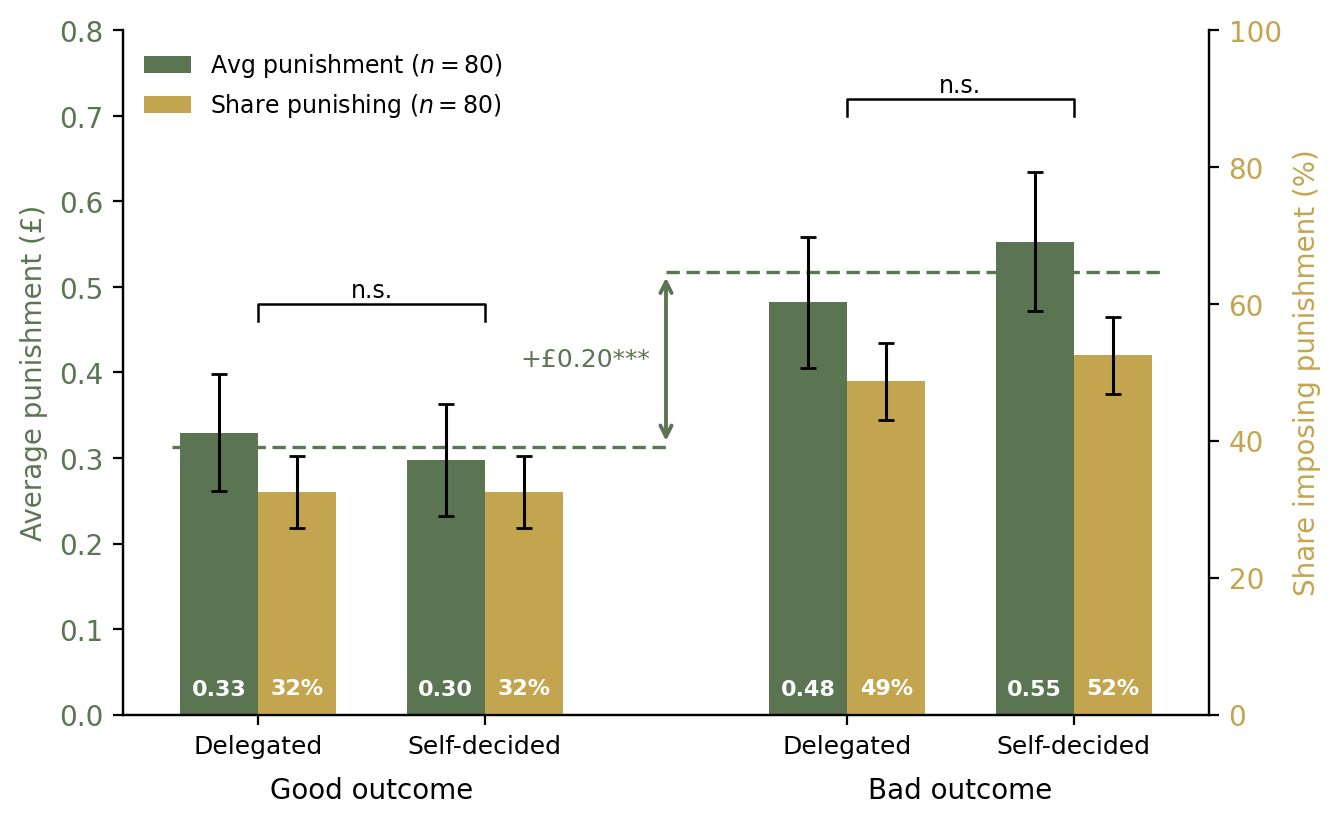
\includegraphics[width=0.6\linewidth]{figures/punishment.png}
    \label{fig:punishment}
    \begin{minipage}{0.85\linewidth}
    \footnotesize
    \textit{Note:} Average punishment chosen by Player~B (solid bars) and average belief about punishment held by Player~A (hollow bars) for each of the four scenarios. Bars are reported in pounds and standard errors are reported as error bars. Beliefs are elicited prior to learning the realized outcome and on the same scale as the punishment decision; the belief overlay is analysed in Section~\ref{sec:mechanism}.
    \end{minipage}
\end{figure}

\paragraph{Equivalence (TOST).} We can refine the negative result with a positive equivalence claim. A two one-sided test (TOST) at the $\pm \pounds 0.20$ bound---against the null that the true insulation effect exceeds $10\%$ of the maximum punishment---rejects in both the bad-outcome cell ($p = 0.012$) and the good-outcome cell ($p < 0.001$). At a tighter $\pm \pounds 0.10$ bound, equivalence cannot be established ($p = 0.332$ for the bad-outcome cell). In our setting we can therefore rule out moderate insulation effects (above $\pounds 0.20$ per cell) with high confidence, but cannot rule out small ones below this bound.

\paragraph{What predicts punishment?} Appendix Table~\ref{tab:reg_punishment} reports a regression of chosen punishment on a delegation indicator, an outcome indicator, their interaction, Player~B's beliefs about Player~A's performance, and a vector of socio-demographic controls. The interaction term is small and statistically insignificant ($p=0.137$), confirming the bivariate result. Punishment is also independent of Player~B's belief about Player~A's performance: across all four cells, Pearson correlations between cell-specific chosen punishment and Player~B's weighted-average belief about Player~A's score are essentially zero ($|r| \le 0.03$, all $p > 0.8$). This rules out the alternative explanation that Player~Bs who think Player~A is more capable systematically punish less (or more); punishment is not driven by performance-conditional inference about Player~A.\footnote{Post-experiment Likert measures provide a tentative attitudes--behavior link. Among the $44$ Player~Bs who passed the attention check and completed the post-experiment questions, those who reported that Player~A should feel more responsible for the decision punish self-made good outcomes more relative to delegated good outcomes (Pearson $r=0.36$, $p=0.015$ between the responsibility Likert and the within-subject difference $\textit{punish\_nodel\_good} - \textit{punish\_del\_good}$); the corresponding pattern in the bad-outcome cell goes in the same direction but is not significant ($r=0.24$, $p=0.114$). When asked directly who should be accountable for AI-generated decisions, $66\%$ of these subjects identified deploying companies as primarily accountable, $18\%$ developers, $14\%$ end-users, and only one named government or regulatory bodies. The sub-sample is small ($n=44$); we treat these patterns as suggestive.}

\paragraph{Interpretation.} The fact that we cannot reject equal punishment for delegated and self-made decisions is consistent with our specific design: because the algorithm is calibrated at the individual level and this calibration is common knowledge, the delegation decision in our setting carries no signal about Player~A's belief in her own ability relative to the algorithm. A natural intention-based punishment motive is therefore muted: Player~B has no obvious basis on which to read the delegation decision as overconfident, lazy, or selfish. By the same token, however, this design choice limits the test of H2 to a setting in which the most studied path through which delegation might insulate from punishment---signal extraction by the third party---is closed off by construction. The complementary reading is that responsibility shifting through delegation may operate more strongly when relative performance is uncertain (as in \citealt{feier_hiding_2022}); we discuss in Section~\ref{conclusion} why a follow-up study that varies relative-performance calibration directly is the natural way to map this margin.

\subsection*{Mechanism: candidate explanations for the H1 reversal} \label{sec:mechanism}

The direction of Result~1 reverses the standard prediction of the responsibility-avoidance literature, in which the prospect of punishment should make delegation \textit{more} attractive, not less. Because the reversal was not preregistered, the analyses in this subsection are exploratory and we treat the supported mechanisms as candidate hypotheses rather than as established. We consider four candidates---anticipated differential punishment (M1), effort to outperform the algorithm (M2), process ownership (M3), and experimenter demand (M4)---and weigh each against the data, taking care to distinguish what we can rule out from what we can only flag as consistent. Before turning to the four candidates, we lay out the belief evidence on which several of them rely, separating beliefs about Player~A's task performance from beliefs about Player~B's punishment.

\paragraph{Performance beliefs.} Both players overestimate Player~A's task performance. The true mean overall score in the first ten rounds is $2.93/10$, while Player~A's weighted-average belief about her own score is $4.76$ (overestimate of $1.84$ score points) and Player~B's weighted-average belief about Player~A's score is $4.32$ (overestimate of $1.40$ score points). The overestimation is therefore not a Player-A-specific or Player-B-specific artefact, but a feature of the elicitation. Performance beliefs do not enter the M1 ruling-out argument below; we report them here as a sanity check on the elicitation rather than as evidence on the mechanism.

\paragraph{Punishment beliefs.} \label{sec:beliefs} After making the delegation decision but before learning the outcome, we elicited Player~A's beliefs about Player~B's punishment in each of the four scenarios. Two patterns emerge. First, Player~As substantially \textit{overestimate} the level of punishment they will face: average expected punishment exceeds average realized punishment in every scenario (Figure~\ref{fig:punishment}, hollow bars). Second, however, Player~As correctly anticipate the \textit{relative} pattern of punishment: they expect no significant difference in punishment between delegated and non-delegated decisions, conditional on outcome---a pattern that closely tracks the actual punishment behavior of Player~B documented in Result~2. \textit{It is this relative-pattern finding---on punishment beliefs alone---that rules out a simple anticipation mechanism for Result~1.} If Player~A had reduced delegation in the \textit{Punishment} because she anticipated being punished more harshly for delegation than for self-made decisions, we would expect to see this asymmetry in the elicited beliefs. We do not.

\paragraph{Within-subject consistency and asymmetric belief patterns.} Despite the weakness of the elicitation, punishment beliefs carry within-subject information. Column~(3) of Table~\ref{tab:del_decision_determinants} reports a Logit regression of delegation on Player~A's belief difference (\textit{no delegation} minus \textit{delegation}) for each outcome, restricted to the \textit{Punishment} condition. Coefficients on both belief differences are positive: a Player~A who expects to be punished more for non-delegation than for delegation in a given outcome is more likely to delegate. The coefficient on the good-outcome belief difference is significant at conventional levels ($1.58$, two-sided $p=0.033$); the coefficient on the bad-outcome belief difference is positive but noisier ($0.94$, two-sided $p=0.21$). The within-subject signal is asymmetric across cells (Figure~\ref{fig:belief_distributions}): the single significant difference between delegators and non-delegators is in the \textit{self decision + good outcome} cell, where delegators expect punishment of $\pounds 0.82$ while non-delegators expect only $\pounds 0.32$ ($t$-test $p=0.006$, Mann-Whitney $p=0.019$); for the other three cells the gap is small and not significant. Because beliefs were elicited after the delegation decision and the elicitation was unincentivised, we cannot rule out that subjects rationalised their choice by holding consistent post-hoc beliefs; the within-subject correlation is consistent with the standard interpretation that anticipated punishment shapes delegation, but does not identify the causal direction.

\begin{figure}[!htbp]
    \centering
    \caption{Player A beliefs about Player B punishment, by delegation choice}
    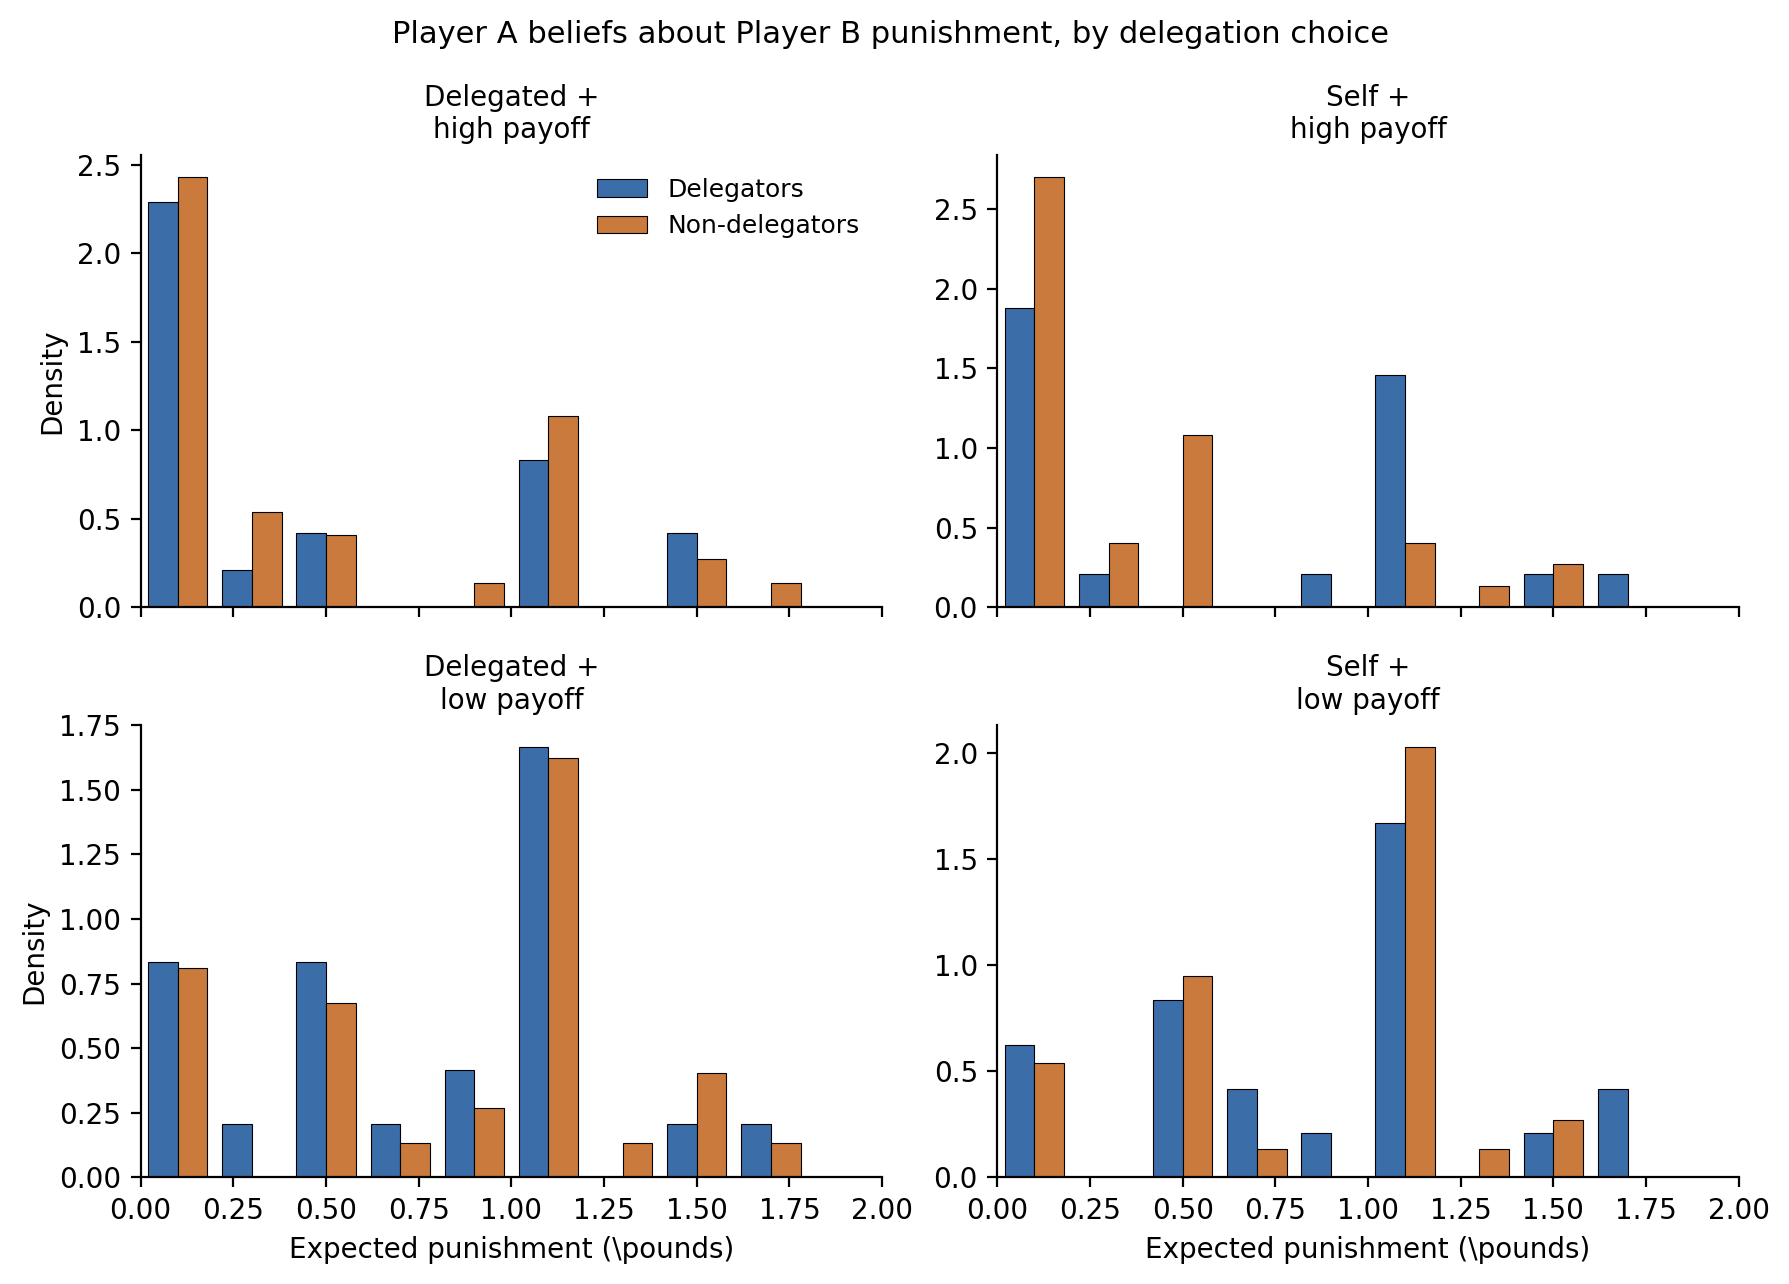
\includegraphics[width=0.85\linewidth]{figures/belief_distributions.png}
    \label{fig:belief_distributions}
    \begin{minipage}{0.9\linewidth}
    \footnotesize
    \textit{Note:} Distribution of Player~A's expected punishment from Player~B in each of the four (delegation, outcome) cells, separately for Player~As who actually delegated (blue) and those who did not (orange). \textit{Punishment} condition, attention-check passers ($n_{\text{deleg}}=24$, $n_{\text{nodeleg}}=37$). The only cell with a statistically significant difference is \textit{self decision + good outcome} (top right): delegators expected $\pounds 0.82$ vs non-delegators $\pounds 0.32$ ($t$-test $p=0.006$).
    \end{minipage}
\end{figure}

\paragraph{(M1) Anticipated punishment for delegation.} A Player~A who expects to be punished more harshly for a delegated decision than for a self-made decision will rationally delegate less when punishment is on the table. The punishment-belief evidence above shows that Player~As do not on average anticipate harsher punishment for delegated decisions, and Player~B does not in fact deliver such punishment (Result~2). M1 is therefore inconsistent with both the elicited beliefs and the realized punishment, and we view this candidate as ruled out by the available evidence.

\paragraph{(M2) Effort exertion to outperform the algorithm.} An alternative mechanism is that the prospect of punishment motivates Player~A to exert greater effort on the final prediction, in the hope of personally producing the high payoff. Although our design controls for relative performance based on the first ten rounds---making the algorithm and Player~A equivalent in expectation on the final prediction---potential punishment could in principle shift Player~A's effort margin. The data are inconsistent with the simple form of this story. Among Player~As who chose not to delegate, those in the \textit{No-Punishment} condition (where punishment is not possible) outperformed those in the \textit{Punishment} condition: $45.5\%$ of non-delegating Player~As in the \textit{No-Punishment} condition earned the high payoff for Player~B, compared to $21.7\%$ in the \textit{Punishment} condition. This difference is not driven by ex-ante performance differences across the first ten rounds (\textit{No-Punishment}: $3.12/10$; \textit{Punishment}: $2.98/10$; two-sided $p=0.66$); the cross-condition mean score in the first ten rounds is $2.93/10$ overall and statistically indistinguishable across conditions (Figure~\ref{fig:performance}), so the M2-relevant gap among non-delegators reflects selection on delegation rather than ex-ante condition differences.\footnote{Measuring performance change as the difference between the average absolute prediction error across the first ten rounds and the absolute prediction error on the final prediction, we find that Player~As in the \textit{No-Punishment} condition improve their performance from rounds~1--10 to round~11, whereas Player~As in the \textit{Punishment} condition do not improve. Because all Player~As across both conditions faced the same image on the final prediction, this differential improvement cannot be attributed to task-specific variation. We caveat that the comparison is between selected non-delegator subsamples, not between random subsets of all Player~As; selection on the very outcome we are measuring is a known limit of this comparison.} Counter-intuitively, increased effort thus appears concentrated among non-delegators in the \textit{No-Punishment} condition, where punishment is \textit{not} on the table---incompatible with a story in which Player~A in the \textit{Punishment} condition tries especially hard to outperform the algorithm in order to avoid punishment.

\begin{figure}[!htbp]
    \centering
    \caption{Performance in the first ten rounds, by treatment}
    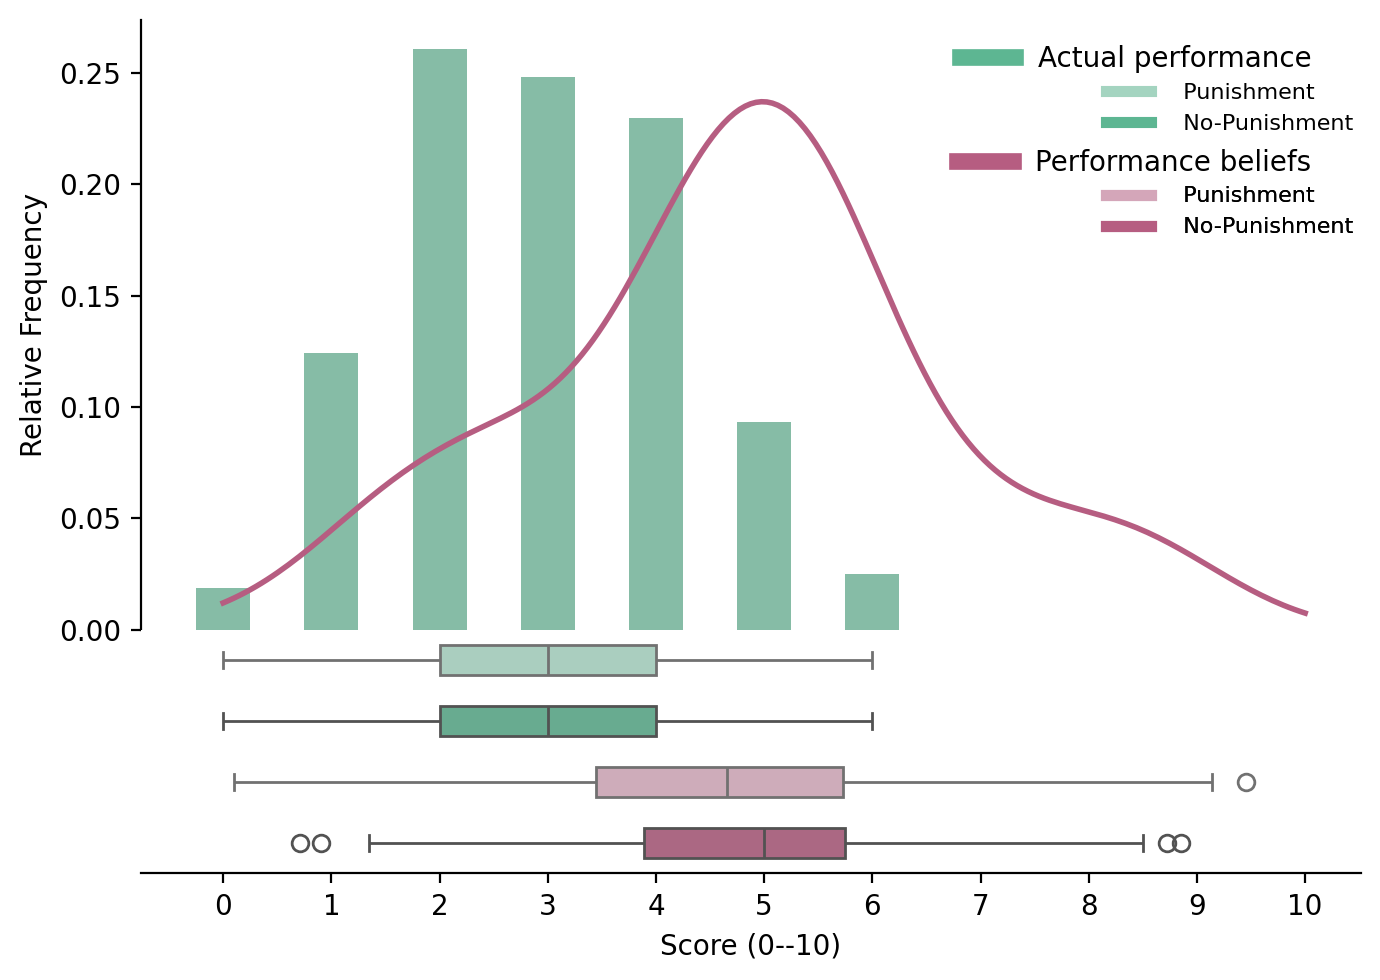
\includegraphics[width=0.75\linewidth]{figures/performance.png}
    \label{fig:performance}
    \begin{minipage}{0.85\linewidth}
    \footnotesize
    \textit{Note:} Distribution of correct predictions (within $10$~lbs of the true weight) over the first ten task rounds, by condition. Average performance is $2.93$ correct out of ten and is statistically indistinguishable across conditions.
    \end{minipage}
\end{figure}

\paragraph{(M3) Process ownership of the outcome.} A third mechanism, suggested by the heterogeneity of the delegation decision with respect to Player~A's performance documented in Result~1 above (and Column~(3) of Table~\ref{tab:del_decision_determinants}), is that Player~As who have a higher subjective probability of producing the high payoff for Player~B prefer to bring about that good outcome themselves rather than via the algorithm. The intuition draws on the psychological-ownership literature: people derive utility from being the proximate cause of a good outcome for another, and this utility is asymmetric with respect to outcomes \citep{steffel_passing_2016}. The data are consistent with this mechanism, but the supporting evidence is thin. The negative relationship between performance and delegation in the \textit{Punishment} condition is what process-ownership predicts: better-performing Player~As, who are more likely to deliver the high payoff, prefer to do so personally. The absence of this relationship in the \textit{No-Punishment} condition is consistent with process ownership being amplified by the moral salience that the punishment possibility introduces. We are explicit, however, that the supporting evidence consists of a single heterogeneity pattern in a 60-subject sub-sample and a comparison of selected non-delegator success rates; the pattern is the most consistent reading of the data we have, but not a confirmed mechanism. A direct test would require a treatment that varies process ownership while holding the punishment possibility fixed---for example, an arm in which the algorithm is presented as Player~A's own ``tool'' rather than as a separate agent.

\paragraph{(M4) Experimenter demand.} A final possibility is that the punishment possibility cues Player~A to behave more conservatively---for instance, to avoid an action (delegation) that the experimental setting itself implicitly frames as morally questionable. We cannot rule this mechanism out with our data. The most we can say is that two implications of a strong demand story are not borne out: if demand were dominant, Player~A's behavior should track elicited beliefs more tightly than it does, and the sharp performance heterogeneity in the \textit{Punishment} condition (better performers delegating less) would be hard to explain. Neither absence is decisive against the demand reading. We discuss the implications, and the design moves that would identify demand directly, in Section~\ref{conclusion}.

\medskip

In sum: M1 (anticipated differential punishment) is inconsistent with the data. M2 (effort to outperform the algorithm) is inconsistent with the data in its simple form. M3 (process ownership) is consistent with the data but supported only by exploratory heterogeneity analysis. M4 (experimenter demand) cannot be separated from M3 with the present design. The most economical reading---the one we adopt with explicit hedges in the Conclusion---is that the morally charged context introduced by the punishment possibility makes Player~A want to be the proximate cause of any good outcome for Player~B, while we acknowledge that an experimenter-demand story can produce qualitatively similar patterns. Disentangling the two is the cleanest direction for follow-up work.
